\section{Task 3}

\textbf{What did we implement?}\\

As the benchmark test are our only way to determine how efficient our program is running we implemented a few more metrics than necessary. We tried to keep the AI and the benchmarking as far separated as possible. To achieve this we adapted our makefile to produce 2 different binaries and try to separate them even more (see next section).\\
Our first two tests are only there to rate the speed of our evaluation function. We can input a map and a time limit and we get as output the amount of evaluation our program could execute in the give time limit.\\
This can be used when we revisit our evaluation functions. The first use is to see if a optimization does really increase the speed and a second one is to control that the evaluations do not become too slow when we implement other rating heuristics. \\\\
The second set of tests is the actual assignment and will analyse our tree search algorithms. For these we can input a map and a depth. As result we get metrics:
\begin{itemize}
	\item The amount of visited nodes
	\item The time taken by the algorithm to find a move
	\item The average amount of evaluations done per second
	\item The time spend evaluating nodes
	\item Percentage of time spend evaluating the leafs 
\end{itemize}
With these parameters we can see where the bottleneck of our system is. For example did it help use to decide to use the paranoid search strategy as we were spending over $99\%$ of our time evaluating leafs for $max^{n}$.\\\\
\textbf{What remains to be solved?}\\

For now, our only concern is that the frequent calling of the timer create an noticeable overhead that is really not necessary for our main program. After all, we save the time at the beginning and end of every leaf evaluation and need to keep track of a counter for the amount of nodes. Our current plans to avoid this, is to search for compiler instruction to only compile those lines of code for out benchmarking project, but not for the AI.\\\\\\ 
\textbf{How are our results?}\\

\textit{The following tests where executed on a ten by ten 2 player board with around 10 stones placed for each player. The OS used is an ubuntu distrubution run in an VM with 2 Gb of RAM and an i7 skylake processor.}\\\\

\begin{tikzpicture}
\begin{axis}[
	height=0.5\textwidth,
	width=\textwidth,
	xlabel=Depth,
	xmin=3,
	xmax=7,
	ylabel=Visited Nodes,
	ymin=0,
]
\addplot table {
	3 549
	4 12733
	5 266765
	6 5556154
	7 96277299
};
\addplot table {
	3 276
	4 2640
	5 19112
	6 138025
	7 968422
};
\end{axis}
\end{tikzpicture}

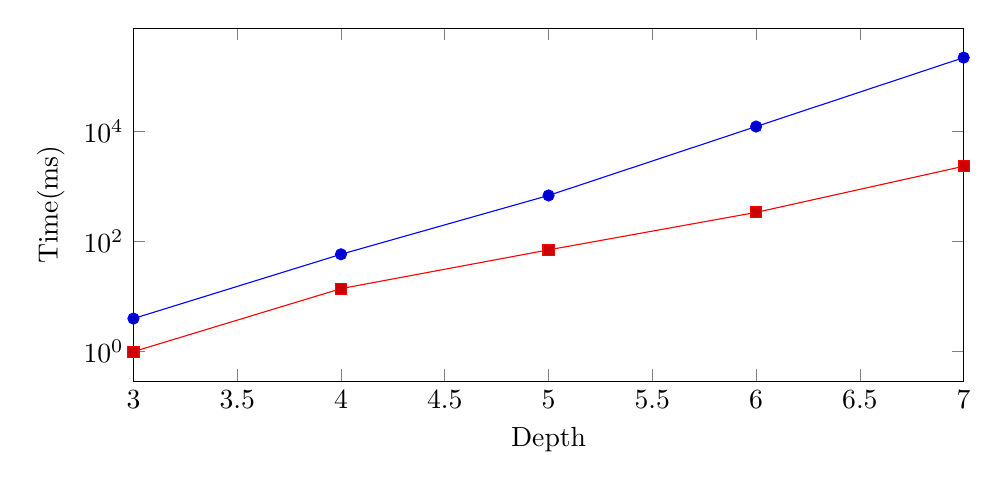
\begin{tikzpicture}
\begin{axis}[
height=0.5\textwidth,
width=\textwidth,
xlabel=Depth,
xmin=3,
xmax=7,
ylabel=Time(ms),
ymin=0,
ymode=log,
]
\addplot table {
	3 4
	4 59
	5 693
	6 12412
	7 222406
};
\addplot table {
	3 1
	4 14
	5 71
	6 341
	7 2353
};
\end{axis}
\end{tikzpicture}

In the first two analysis we compare minimax with alphabeta-pruning. As the amount of nodes visited and the time take to execute the algorithms result in similar graph, we plotted the second one on a logscale. \\
In the first graph we see how much more efficient alphabeta-pruning is in comparision to minimax. In the second graph that impression of superiority shrinks, but we can see much better that there is already a significant difference in small game trees.\\
These result were expected as minimax is in $O(b^{d})$ and alphabeta-pruning's average case runtime is in $O(b^{\frac{3d}{4}})$.\\\\

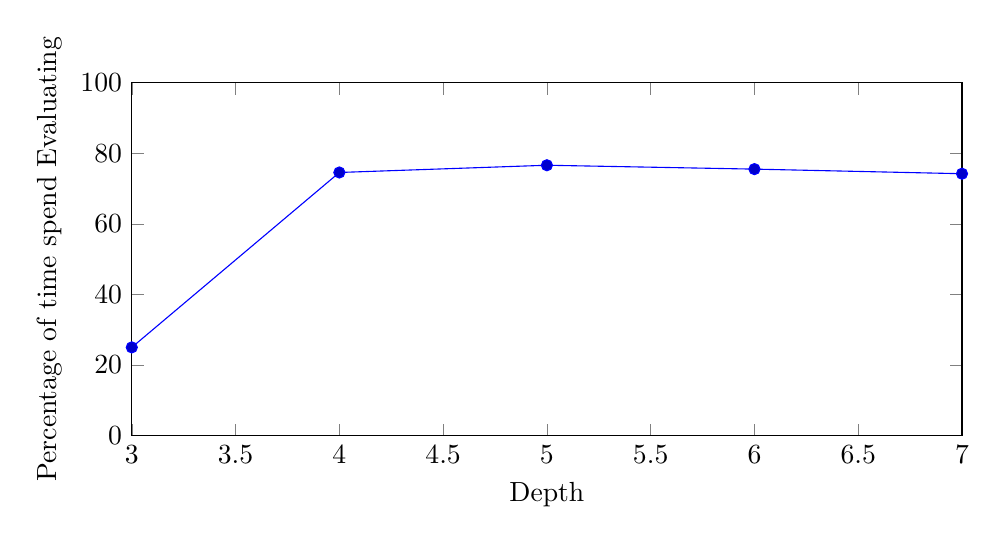
\begin{tikzpicture}
\begin{axis}[
height=0.5\textwidth,
width=\textwidth,
xlabel=Depth,
xmin=3,
xmax=7,
ylabel=Percentage of time spend Evaluating,
ymin=0,
ymax=100,
]
\addplot table {
	3 25
	4 74.57
	5 76.62
	6 75.52
	7 74.2183
};
\end{axis}
\end{tikzpicture}
We also found out that we spend about 75\% of the time evaluating the leafs. How good or bad that value is remains to be seen.\\
We got this number down from 80\% in just about an one our of pruning, and some more performance boosts should be expected.\\\\

\begin{tikzpicture}
\begin{axis}[
height=0.5\textwidth,
width=\textwidth,
xlabel=Depth,
xmin=4,
xmax=10,
ylabel=Evaulations per second,
ymin=0,
]
\addplot table {
	4 158500
	5 244714
	6 132173
	7 247167
	8 245745
	9 259510
	10 196997
};
\end{axis}
\end{tikzpicture}
This last graph shows something interesting. While the evaluations per second remain constant to a certain degree with increasing depth, as they should be, they seem to go up and down. It seems as if we do take more time analysing a board after we have done a move than if we analyse after our enemy has done so. This seems logical as we should have more stones on the board after our own turn, but the changes are quite significant. We might use this information when implementing iterative deepening, to skip some specific depth if we think we have enough time to do so and can risk it.
